\chapter{Analisi dei requisiti}\label{ch:requirements}
  In questo capitolo saranno enunciati ed analizzati i requisiti del progetto realizzato per questa tesi.

  Nella~\Cref{part:background} è stato più volte sottolineato che il linguaggio Protelis si appoggia alla piattaforma JVM per la sua esecuzione.
  Al momento della scrittura, l'unico supporto da parte delle tecnologie browser per Java ritenuto stabile era dato dal plugin per le Applet API\@.
  Tale plugin è stato deprecato da alcuni anni~\cite{jep289} a seguito del rilascio di Java 9;
  la quasi totalità dei browser ne ha ormai dismesso la compatibilità o lo faranno a breve.
  si assume già in questa fase, dunque, che realizzare un'applicazione web solamente client-side sia, al momento, impraticabile.

  Di seguito saranno dunque distinti i requisiti per il server esecutore dai requisiti dell'applicazione front-end che svolgerà il ruolo di client.

  \section{Requisiti del client}
    L'obiettivo principale di questa tesi è progettare un sistema in grado di permettere all'utente di iniziare a utilizzare un linguaggio aggregato come Protelis richiedendo meno configurazioni possibile.
    La componente che deve interfacciarsi con l'utente, il quale si assume essere inesperto della piattaforma, dovrebbe astrarre la maggior parte della complessità e modellare esclusivamente le funzionalità che l'utente potrà utilizzare.

    \subsection{Requisiti funzionali}

      \begin{description}
        \item[Nessun setup]
          Essendo orientato alla sperimentazione con il linguaggio, l'esperienza d'uso deve essere il più semplice possibile.
          In particolare, nel prototipo non deve essere necessario configurare una rete di alcun tipo per poter realizzare codice aggregato ed eseguirlo.
        \item[Modificare il programma]
          Per quanto possa essere utile avere codice di esempio già inserito nel campo di testo, l'applicazione web deve permettere all'utente di sperimentare con i costrutti del linguaggio, avendo la possibilità di scrivere il proprio codice nell'editor.
          Tale editor deve offrire per quanto possibile un'esperienza di scrittura che ricorda quella di un editor di codice desktop.
        \item[Lanciare l'esecuzione]
          L'applicazione deve permettere di lanciare il codice scritto dall'utente su una rete predeterminata di dispositivi.
          Tale rete deve essere trasparente all'utente.
        \item[Visualizzare l'esecuzione]
          L'applicazione deve permettere di osservare graficamente il progresso dell'esecuzione del codice scritto dall'utente.
        % \item[Terminare l'esecuzione] % TODO
        %   Tramite un apposito controllo, l'interfaccia dell'applicazione deve permettere di terminare l'esecuzione della simulazione.
        % TODO: altro?
      \end{description}

    \subsection{Requisiti non funzionali}

      \begin{description}
        \item[Single-Page Application]
          L'applicativo web deve presentarsi come una singola pagina, gestendo tutte le interazioni dell'utente senza appoggiarsi al server.
          Deve connettersi al backend solo per l'esecuzione del codice inserito.
        \item[Agnostico rispetto al backend]
          La rete dispositivi a cui si collega per l'esecuzione deve poter essere reale o virtuale senza che questo influenzi l'esperienza utente con il frontend.
          Le tecnologie utilizzate per l'implementazione del backend devono essere trasparenti al client.
        \item[Efficienza]
          L'esecuzione non deve appesantire il dispositivo client su cui esegue.
          Deve sfruttare in modo efficace le risorse messe a disposizione dalla macchina dell'utente, delegando al server solo le operazioni computazionalmente più pesanti.
        \item[Responsive, ma desktop-first]
          L'applicazione ha come destinazione d'uso il desktop, dunque non è necessaria un'interfaccia \emph{mobile-first}.
          È comunque necessario che il layout della pagina sia \emph{responsive}, ossia possa adattarsi a schermi di differenti misure e proporzioni.
      \end{description}

  \section{Requisiti del server}
    La componente server di questo progetto non deve interfacciarsi direttamente con l'utente, bensì fornire delle API generiche per l'esecuzione di codice Protelis proveniente dal client.

    \subsection{Requisiti funzionali}

    \begin{description}
      \item[Esecuzione di codice Protelis]
        Il server deve poter eseguire codice Protelis ricevuto tramite le proprie API esposte in rete.
        In particolare, il server deve essere in grado di generare reti simulate di dispositivi su cui eseguire il codice \emph{on-demand}.
      \item[Supporto a più esecuzioni contemporanee]
        Il server deve permettere a più utenti di lavorare con il sistema contemporaneamente.
        In particolare, deve essere in grado di gestire più simulazioni, ciascuna distinta dalle altre e associata al client che l'ha richiesta.
      \item[Mantenimento della connessione]
        Il server deve essere in grado di mantenere una connessione bidirezionale stabile con ciascun client, in modo da permettere al client di ottenere aggiornamenti sullo stato dell'esecuzione.
    \end{description}

    \subsection{Requisiti non funzionali}

    \begin{description}
      \item[Scalabilità]
        Il sistema deve essere aperto alla possibilità di essere scalato efficacemente.
        In particolare, non è necessario che il prototipo sia in grado di scalare autonomamente, ma deve permettere l'introduzione di un eventuale orchestratore senza particolare difficoltà.
      \item[Protocollo di connessione efficiente]
        Il server deve esporre le proprie API tramite un protocollo efficiente dal punto di vista delle performance, non andando a limitare in modo sensibile la velocità con cui il frontend viene informato dei progressi dell'esecuzione.
        Inoltre, tali API dovrebbero permettere di sostituire lo standard di comunicazione senza la necessità di effettuare modifiche notevoli nel motore.
        Infine, il protocollo utilizzato dal prototipo dovrebbe essere supportato da quante più piattaforme possibile (con particolare attenzione ai browser più usati).
    \end{description}

    \improvement[inline]{Il capitolo dovrebbe essere espanso un po'? Magari aggiungendo maggiori dettagli o diagrammi?}

    \begin{figure}[htbp]
      \centering
      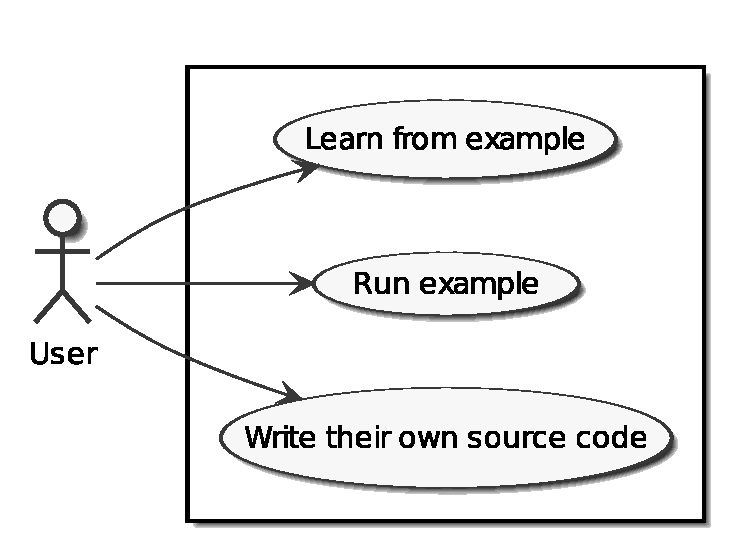
\includegraphics[width=.6\textwidth]{res/uml/use-cases-frontend.eps}%
      \caption{Il diagramma UML rappresenta i casi d'uso principali dell'interfaccia}%
      \label{fig:uml-use-case}
    \end{figure}
